\chapter{Séparer les mélanges}\label{ch:g3:separating-mixtures}

Après un orage, les flaques de la route sont brunes~: de l'eau de pluie
mélangée à de la terre, du sable et des débris de feuilles. Pourtant,
l'eau qui sort du robinet de la cuisine est limpide, et elle aussi a été
de la pluie, avant de couler dans une rivière. Comment rendre propre une
eau boueuse~? Ce qui a été mélangé peut être séparé. Ce chapitre montre
comment, une méthode après l'autre.

\begin{recall}
\omterm{def:g2:mixing-and-dissolving:mix}{Mélanger}, c'est mettre des choses différentes ensemble. Un solide comme
le sucre ou le sel \omterm{def:g2:mixing-and-dissolving:dissolve}{se dissout} dans l'eau~: il disparaît à la vue, et le
liquide limpide obtenu est une solution. Un solide dissous est toujours
là~: quand l'eau sèche, le solide reste. Le sable et la terre ne se
dissolvent pas (\cref{ch:g2:mixing-and-dissolving}).
\end{recall}

\section{Trier à la main et tamiser}

Quand les morceaux d'un \omterm{def:g2:mixing-and-dissolving:mix}{mélange} sont assez gros pour être vus et
ramassés, le plus simple pour les séparer est de les trier à la main~:
on peut retirer un à un les raisins secs du muesli. Quand il y a trop de
morceaux, un tamis fait le tri à notre place.

\begin{definition}[Tamisage]\label{def:g3:separating-mixtures:sieve}
Le \emph{tamisage}\index{tamisage} consiste à séparer les morceaux d'un
\omterm{def:g2:mixing-and-dissolving:mix}{mélange} selon leur taille, avec un tamis~: un filet ou une plaque pleine
de trous. Les petits morceaux passent par les trous~; les gros restent
dans le tamis.
\end{definition}

\begin{example}[Gravier et sable]\label{ex:g3:separating-mixtures:gravel}
Un maçon secoue un \omterm{def:g2:mixing-and-dissolving:mix}{mélange} de gravier et de sable au-dessus d'un tamis.
Le sable fin passe à travers et forme un tas en dessous~; le gravier
reste sur le grillage.
\end{example}

\begin{omfigure}
\begin{tikzpicture}[font=\small]
  % the sieve: a mesh bowl
  \fill[pattern=crosshatch, pattern color=black!45] (-1.6,2.6) arc[start angle=180,
    end angle=360, x radius=1.6, y radius=0.7] -- cycle;
  \draw[black!70, line width=0.8pt] (-1.6,2.6) arc[start angle=180, end angle=360,
    x radius=1.6, y radius=0.7];
  \draw[black!70, line width=0.8pt] (-1.75,2.6) -- (1.75,2.6);
  \draw[black!70, line width=1.4pt] (1.75,2.6) -- (3.0,2.85);
  % gravel kept in the sieve
  \foreach \x/\y/\r in {-0.9/2.25/0.17,-0.45/2.12/0.2,0.05/2.08/0.18,0.5/2.13/0.21,
                        0.95/2.28/0.16,-0.2/2.42/0.15,0.3/2.43/0.17}
    \fill[black!45, draw=black!65] (\x,\y) circle (\r);
  % sand falling
  \foreach \x/\y in {-0.4/1.6,0.1/1.4,0.4/1.7,-0.15/1.15,0.25/1.0,-0.5/0.95,0.0/0.75}
    \fill[orange!60!brown] (\x,\y) circle (0.05);
  % the heap of sand in a bowl
  \fill[orange!45!brown!70] (-1.0,0.12) .. controls (-0.5,0.55) and (0.5,0.55)
    .. (1.0,0.12) -- cycle;
  \draw[black!70, line width=0.8pt] (-1.5,0.5) .. controls (-1.3,0) and (1.3,0)
    .. (1.5,0.5);
  \node[anchor=west] at (2.0,2.2) {le gravier reste dans le tamis};
  \node[anchor=west] at (2.0,1.25) {le sable passe par les trous};
  \node[anchor=west] at (2.0,0.3) {un tas de sable};
\end{tikzpicture}

{\small \omterm{def:g3:separating-mixtures:sieve}{Tamisage} d'un \omterm{def:g2:mixing-and-dissolving:mix}{mélange} de gravier et de sable~: les morceaux sont
triés selon leur taille.}
\end{omfigure}

\begin{omfigure}
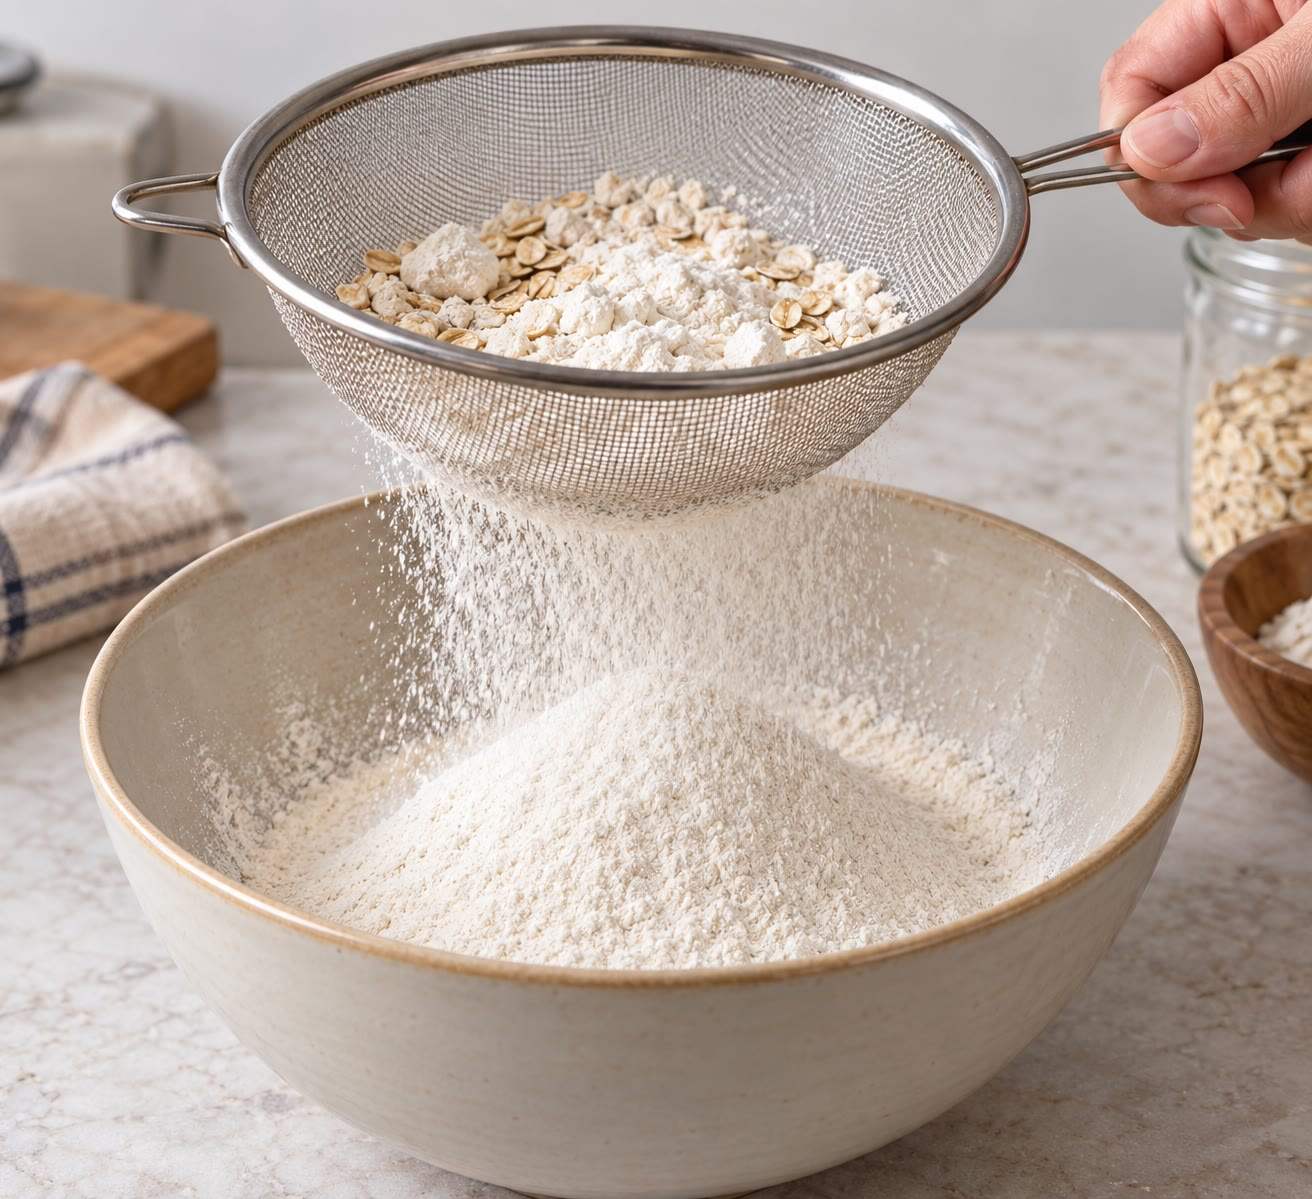
\includegraphics[width=0.55\linewidth]{images/book1/ai/g3-kitchen-sieve.jpg}

{\small Un tamis de cuisine~: la farine fine passe, les grumeaux restent.}
\end{omfigure}

\section{Laisser reposer et transvaser}

\begin{definition}[Décantation et transvasement]\label{def:g3:separating-mixtures:decant}
On peut laisser reposer un \omterm{def:g2:mixing-and-dissolving:mix}{mélange} d'eau et d'un solide qui ne \omterm{def:g2:mixing-and-dissolving:dissolve}{se
dissout} pas~: le solide descend lentement au fond. C'est la
\emph{décantation}\index{decantation@décantation}. Une fois le solide déposé, on
peut verser doucement l'eau claire du dessus dans un autre récipient, en
laissant le solide au fond~: c'est le
\emph{transvasement}\index{transvasement}.
\end{definition}

\begin{omfigure}
\begin{tikzpicture}[font=\small]
  % 1: stirred, cloudy
  \pic at (0,0) {beaker={0.7}{brown!28}};
  \foreach \x/\y in {-0.5/0.3,-0.2/0.6,0.3/0.4,0.5/0.9,-0.4/1.0,0.1/1.2,0.4/0.15,
                     -0.1/0.25,0.2/0.8,-0.55/0.7}
    \fill[brown!60] (\x,\y) circle (0.03);
  \node[anchor=north, align=center] at (0,-0.15) {remué~:\\ trouble};
  \draw[->, thick, omProp] (1.1,1.0) -- (2.4,1.0);
  % 2: settled
  \pic at (3.5,0) {beaker={0.7}{omWater!80}};
  \fill[brown!60] (2.7,0) rectangle (4.3,0.25);
  \draw[omGlass, line width=0.7pt] (2.7,0.25) -- (2.7,0) -- (4.3,0) -- (4.3,0.25);
  \node[anchor=north, align=center] at (3.5,-0.15) {laissé au repos~:\\ la terre s'est déposée};
  \draw[->, thick, omProp] (4.6,1.0) -- (5.9,1.0);
  % 3: decanted
  \pic at (7.0,0) {beaker={0.1}{omWater!80}};
  \fill[brown!60] (6.2,0) rectangle (7.8,0.25);
  \draw[omGlass, line width=0.7pt] (6.2,0.25) -- (6.2,0) -- (7.8,0) -- (7.8,0.25);
  \pic at (9.2,0) {beaker={0.58}{omWater!80}};
  \node[anchor=north, align=center] at (8.1,-0.15) {transvasé~: l'eau claire\\ à droite, la terre reste au fond};
\end{tikzpicture}

{\small \omterm{def:g3:separating-mixtures:decant}{Décantation}, puis \omterm{def:g3:separating-mixtures:decant}{transvasement} d'un \omterm{def:g2:mixing-and-dissolving:mix}{mélange} de terre et d'eau.}
\end{omfigure}

\begin{remark}[La décantation prend du temps]\label{rem:g3:separating-mixtures:time}
Les gros grains lourds se déposent en quelques minutes~; une argile très
fine peut mettre un jour ou plus, et l'eau reste un peu trouble pendant
ce temps. Le \omterm{def:g3:separating-mixtures:decant}{transvasement} n'enlève jamais tous les grains~: un léger
trouble part avec l'eau.
\end{remark}

\section{Filtrer}

\begin{definition}[Filtration et filtrat]\label{def:g3:separating-mixtures:filter}
La \emph{filtration}\index{filtration} consiste à verser un \omterm{def:g2:mixing-and-dissolving:mix}{mélange} à
travers un filtre~: une feuille de papier, un tissu ou une couche de
sable dont les trous sont trop petits pour laisser passer les morceaux
solides. Le solide reste sur le filtre~; le liquide limpide qui passe à
travers s'appelle le \emph{filtrat}\index{filtrat}.
\end{definition}

\begin{omfigure}
\begin{tikzpicture}[font=\small, scale=1.4]
  \pic[transform shape] at (0,0) {beaker={0.35}{omWater!80}};
  \pic[transform shape] at (0,1.4) {funnel={brown!55}};
  % muddy water waiting in the paper cone, above the soil
  \fill[brown!25] (-0.411,2.45) -- (0.411,2.45) -- (0.722,2.8) -- (-0.722,2.8) -- cycle;
  % drops of filtrate
  \foreach \y in {1.15,0.95} \fill[omDef!50] (0,\y) circle (0.04);
  \draw[<-, omProp, thick] (0.75,2.6) -- (2.0,2.9) node[right, text=black]
    {papier filtre dans un entonnoir};
  \draw[<-, omProp, thick] (0.25,2.15) -- (2.0,2.2) node[right, text=black]
    {la terre reste sur le papier};
  \draw[<-, omProp, thick] (0.85,0.4) -- (2.0,0.6) node[right, text=black]
    {le filtrat~: de l'eau limpide};
\end{tikzpicture}

{\small \omterm{def:g3:separating-mixtures:filter}{Filtration} d'une eau boueuse à travers un filtre en papier.}
\end{omfigure}

\begin{inthelab}[Filtrer une eau boueuse]
L'enseignant plie une feuille ronde de papier filtre en cône et la place
dans un entonnoir en verre, au-dessus d'un bécher. On verse l'eau
boueuse dans le cône, peu à peu, sans jamais dépasser le bord du papier.
De l'eau limpide goutte dans le bécher~; la terre forme une couche brune
sur le papier. Si le \omterm{def:g3:separating-mixtures:filter}{filtrat} est trouble, c'est que le papier est
déchiré ou que l'eau a débordé.
\end{inthelab}

\begin{proposition}[Un filtre n'arrête pas ce qui est dissous]\label{prop:g3:separating-mixtures:dissolved}
Un filtre retient les morceaux solides qui ne sont pas dissous. Il ne
retient pas ce qui est dissous~: de l'eau salée versée sur un filtre en
ressort tout aussi salée, et du thé sucré tout aussi sucré.
\end{proposition}

\begin{omfigure}
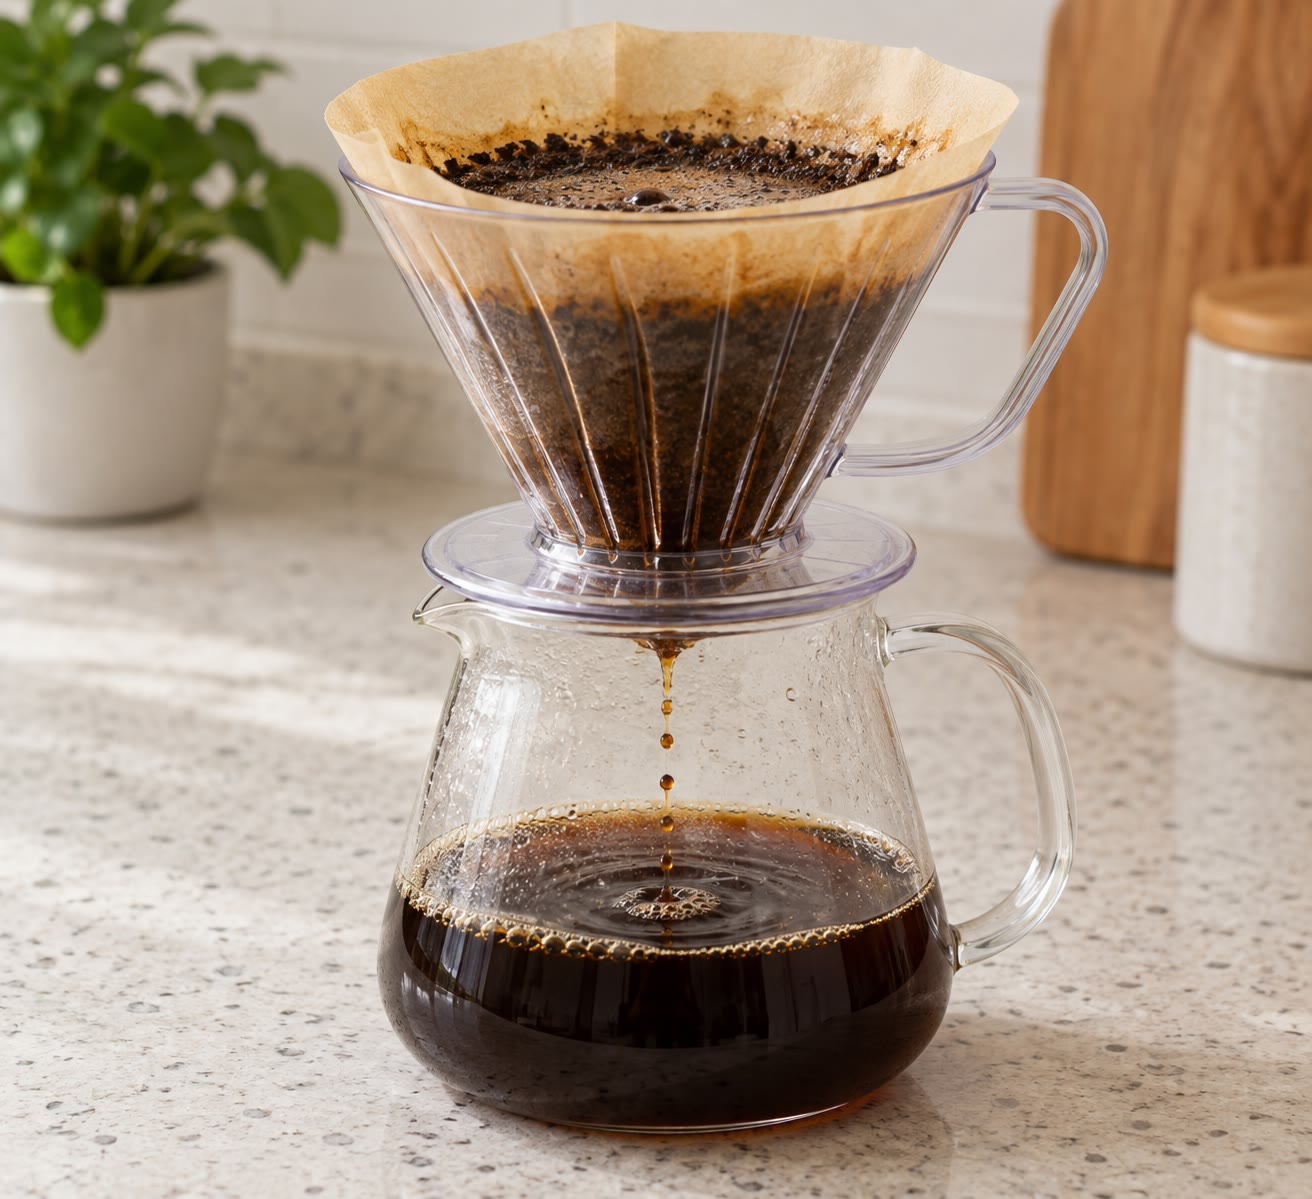
\includegraphics[width=0.5\linewidth]{images/book1/ai/g3-coffee-filter.jpg}

{\small Faire du café, c'est filtrer~: le marc reste dans le papier, le
café est le \omterm{def:g3:separating-mixtures:filter}{filtrat}.}
\end{omfigure}

\section{Faire s'évaporer l'eau}

\begin{definition}[Évaporation]\label{def:g3:separating-mixtures:evaporate}
Pour récupérer un solide dissous dans l'eau, on laisse l'eau sécher, au
soleil ou sur un chauffage doux~: c'est
l'\emph{évaporation}\index{evaporation@évaporation}. L'eau part dans l'air~; le
solide reste dans la coupelle.
\end{definition}

\begin{example}[Le sel de l'eau salée]\label{ex:g3:separating-mixtures:salt}
On verse un peu d'eau salée dans une coupelle peu profonde, posée sur
le rebord d'une fenêtre ensoleillée. Quelques jours plus tard, il n'y a
plus d'eau, seulement une croûte blanche de sel~: le sel qui était
dissous.
\end{example}

\begin{omfigure}
\begin{tikzpicture}[font=\small, scale=1.4]
  \pic[transform shape] at (0,0) {hotplate};
  \pic[transform shape] at (0,0) {evapdish={omWater!80}};
  \node[anchor=north, align=center] at (0,-0.6) {eau salée,\\ chauffée doucement};
  \draw[->, thick, omProp] (1.5,0.3) -- (3.0,0.3) node[midway, above, text=black]
    {plus tard};
  \pic[transform shape] at (4.5,0) {hotplate};
  \pic[transform shape] at (4.5,0) {evapdish={white!85!black}};
  \foreach \x in {-0.45,-0.25,-0.05,0.15,0.35}
    \fill[white, draw=black!45, line width=0.2pt] (4.5+\x,0.12) rectangle ++(0.09,0.06);
  \node[anchor=north, align=center] at (4.5,-0.6) {plus d'eau~:\\ des cristaux de sel};
  \foreach \x in {-0.3,0,0.3} \draw[->, black!45, decorate,
    decoration={snake, amplitude=0.6pt, segment length=4pt}] (\x,0.7) -- (\x,1.4);
  \node[anchor=south] at (0,1.4) {l'eau part dans l'air};
\end{tikzpicture}

{\small L'\omterm{def:g3:separating-mixtures:evaporate}{évaporation} au laboratoire~: l'enseignant chauffe doucement la
coupelle sur une plaque chauffante. Le sel reste dans la coupelle.}
\end{omfigure}

\section{Quelle méthode pour quel mélange~?}

\begin{method}[Choisir une séparation]\label{met:g3:separating-mixtures:choose}
Pour séparer un \omterm{def:g2:mixing-and-dissolving:mix}{mélange}, pose-toi ces questions~:
\begin{enumerate}
  \item Les morceaux sont-ils gros et de tailles différentes~? Trie à la
        main, ou tamise.
  \item Y a-t-il, dans un liquide, un solide qui ne \omterm{def:g2:mixing-and-dissolving:dissolve}{se dissout} pas~?
        Laisse décanter puis transvase, ou filtre pour avoir une eau plus
        claire.
  \item Y a-t-il un solide dissous dans le liquide~? Fais évaporer le
        liquide~: le solide reste.
\end{enumerate}
Il faut souvent plusieurs étapes, l'une après l'autre.
\end{method}

\begin{example}[Sable, sel et eau]\label{ex:g3:separating-mixtures:three}
Un bocal contient de l'eau avec du sable et du sel. Le sel s'est
dissous~; le sable, non.
\begin{enumerate}
  \item On filtre~: le sable reste sur le papier.
  \item Le \omterm{def:g3:separating-mixtures:filter}{filtrat} est limpide, mais c'est de l'eau salée. On le fait
        évaporer~: le sel reste dans la coupelle.
\end{enumerate}
Deux méthodes, l'une après l'autre, permettent de récupérer le sable et
le sel.
\end{example}

\begin{example}[De l'eau propre à partir d'une rivière]\label{ex:g3:separating-mixtures:plant}
Une usine de traitement de l'eau rend l'eau de rivière potable en
plusieurs étapes~:
\begin{enumerate}
  \item l'eau de la rivière passe à travers des dégrilleurs, de grandes
        grilles qui arrêtent les branches, les feuilles et les
        plastiques~: c'est une sorte de \omterm{def:g3:separating-mixtures:sieve}{tamisage}~;
  \item elle repose dans de grands bassins où la boue se dépose au
        fond~;
  \item elle est filtrée à travers d'épaisses couches de sable qui
        retiennent les grains les plus fins~;
  \item on ajoute une toute petite quantité d'un produit qui tue les
        microbes, pour que l'eau reste saine dans les tuyaux.
\end{enumerate}
\end{example}

\begin{omfigure}
\begin{tikzpicture}[font=\small, node distance=0.45cm,
    box/.style={draw=omDef, fill=omDef!6, rounded corners=2pt, align=center,
      minimum height=1.15cm, text width=2.0cm}]
  \node[box] (r) {eau de\\ rivière};
  \node[box, right=of r] (s) {grilles\\ (tamisage)};
  \node[box, right=of s] (t) {bassins de\\ décantation};
  \node[box, right=of t] (f) {filtres\\ à sable};
  \node[box, right=of f] (g) {microbes\\ tués};
  \foreach \a/\b in {r/s,s/t,t/f,f/g} \draw[->, thick, omProp] (\a) -- (\b);
  \node[below=0.15cm of s, font=\footnotesize, align=center] {branches,\\ plastiques};
  \node[below=0.15cm of t, font=\footnotesize, align=center] {boue};
  \node[below=0.15cm of f, font=\footnotesize, align=center] {grains fins};
  \draw[->, thick, omProp] (g.south) -- ++(0,-0.8) node[below] {vers les robinets};
\end{tikzpicture}

{\small Les étapes d'une usine de traitement de l'eau. Sous chaque
étape~: ce qu'elle enlève.}
\end{omfigure}

\begin{omfigure}
\begin{minipage}[t]{0.48\linewidth}\centering
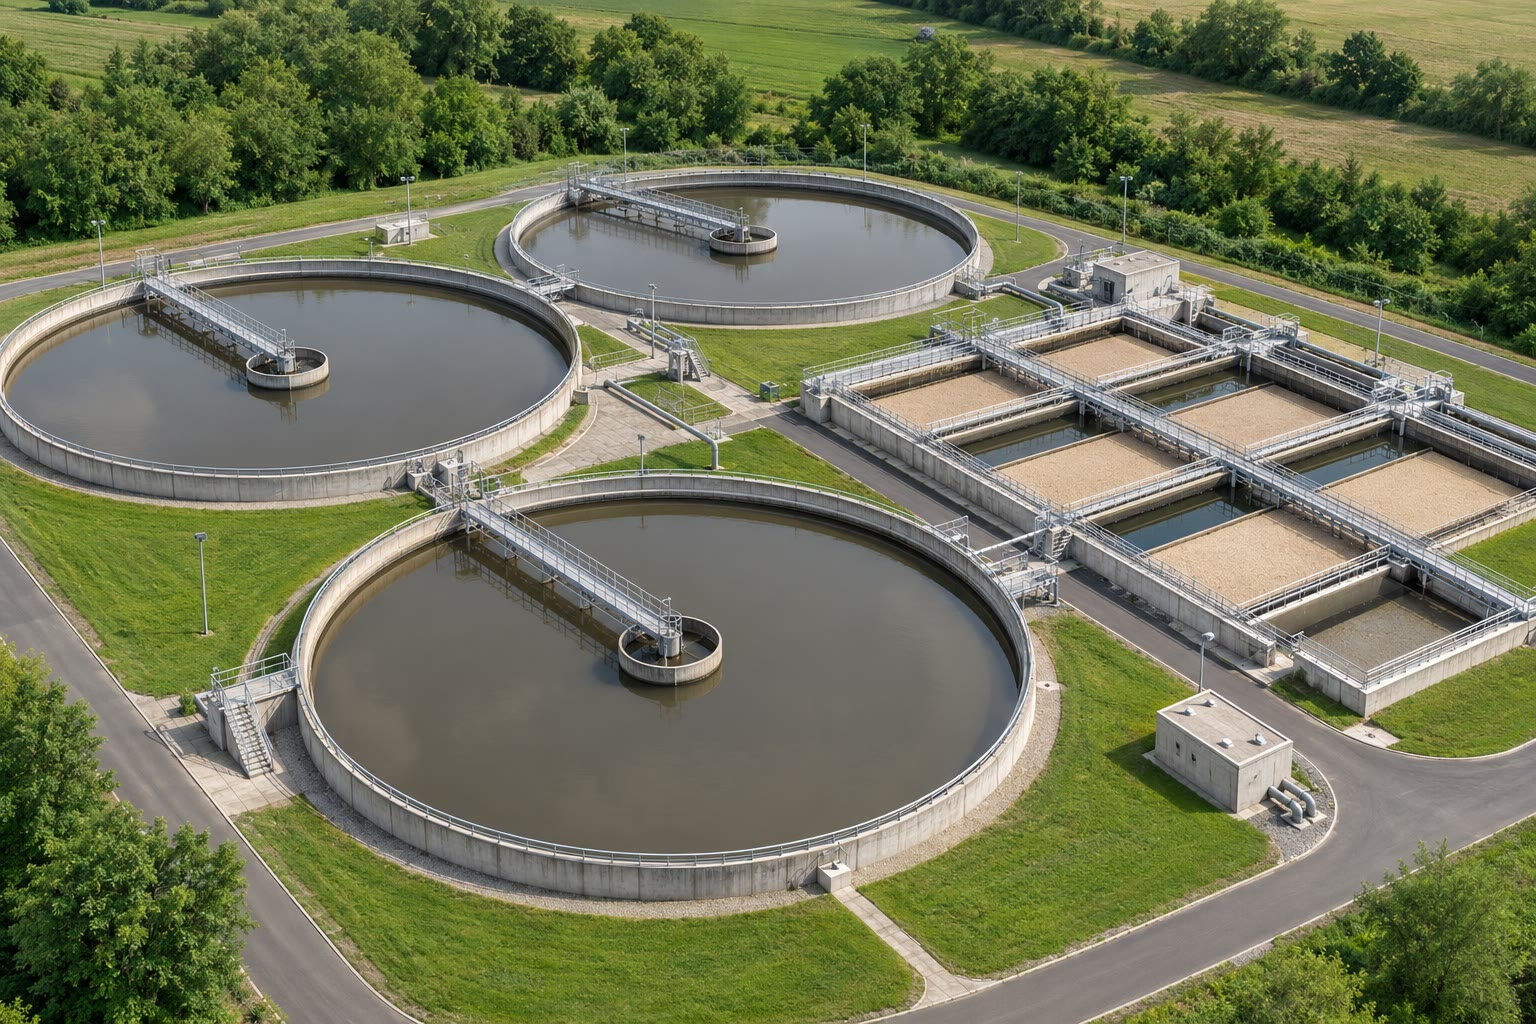
\includegraphics[width=\linewidth,height=4.6cm,keepaspectratio]{images/book1/ai/g3-settling-tanks.jpg}

{\small Les bassins de \omterm{def:g3:separating-mixtures:decant}{décantation} d'une usine de traitement de l'eau.}
\end{minipage}\hfill
\begin{minipage}[t]{0.48\linewidth}\centering
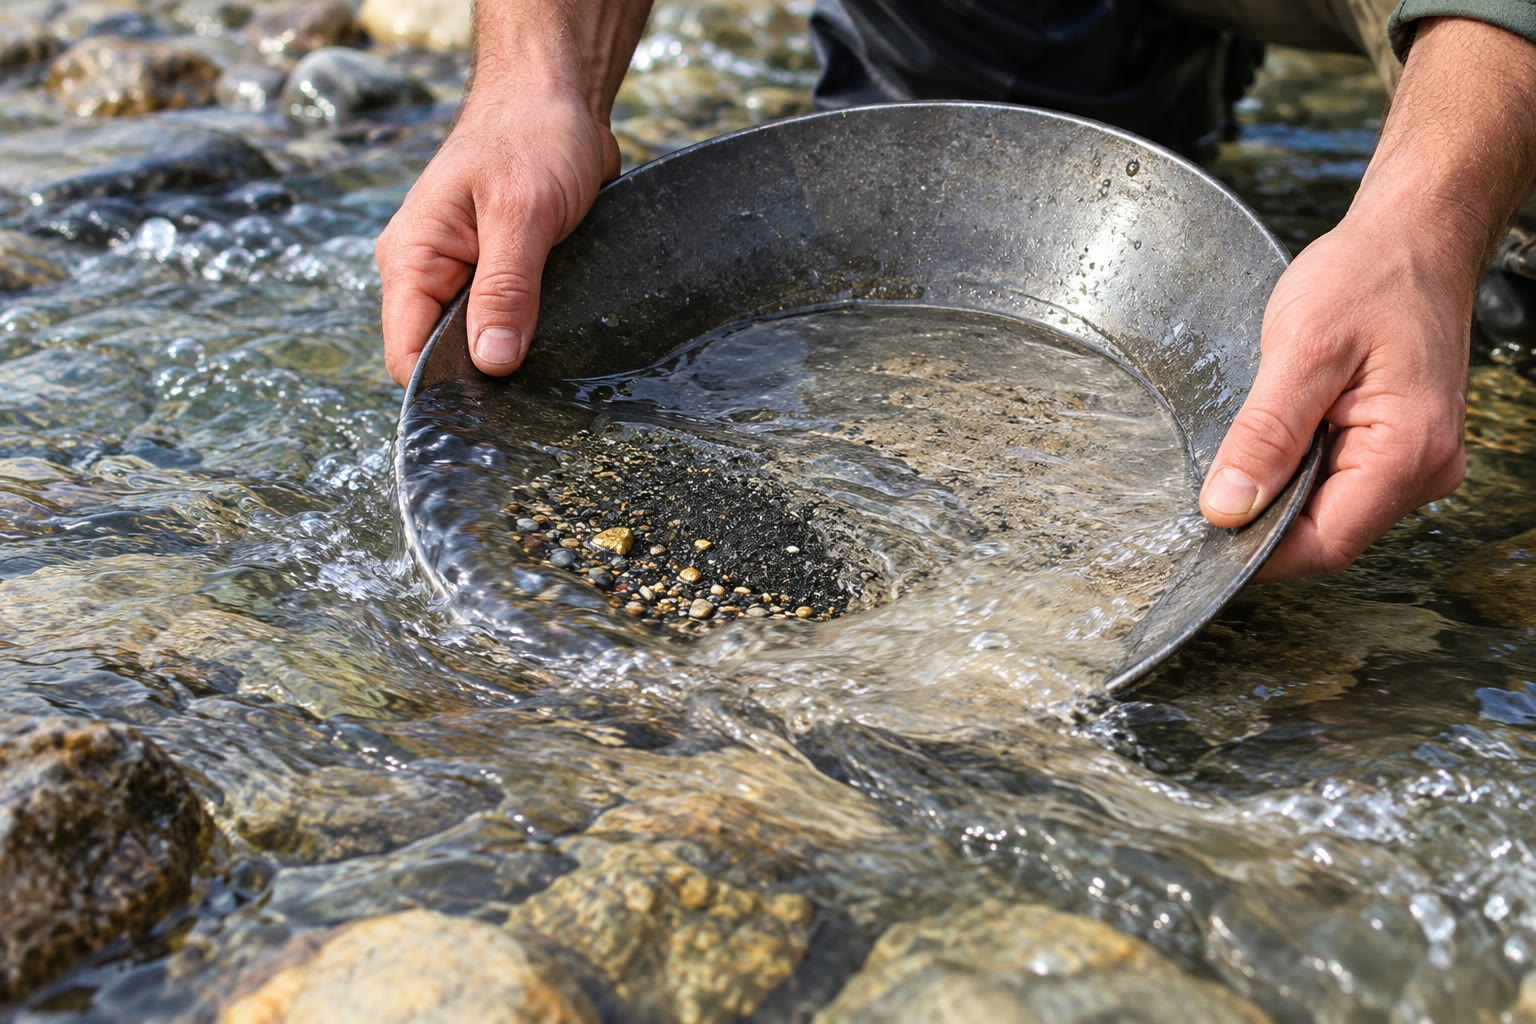
\includegraphics[width=\linewidth,height=4.6cm,keepaspectratio]{images/book1/ai/g3-gold-panning.jpg}

{\small L'orpaillage~: l'eau de la rivière emporte le sable léger~; les
grains lourds restent dans la batée.}
\end{minipage}
\end{omfigure}

\begin{remark}[Limpide ne veut pas toujours dire propre]\label{rem:g3:separating-mixtures:clean}
Une eau filtrée peut sembler parfaitement limpide et contenir encore
des substances dissoutes, et des microbes bien trop petits pour être
vus. C'est pourquoi personne ne boit l'eau d'une flaque ou d'un
ruisseau, même après l'avoir filtrée.
\end{remark}

\section{Exercices}

\begin{exercise}[$\star$]\label{exo:g3:separating-mixtures:1}
Quelle méthode utiliserais-tu pour séparer des petits pois de grains de
riz~?
\end{exercise}

\begin{exercise}[$\star$]\label{exo:g3:separating-mixtures:2}
On laisse un verre d'eau boueuse sur une table pendant une heure. Que
devient la terre~? Comment s'appelle ce phénomène~?
\end{exercise}

\begin{exercise}[$\star$]\label{exo:g3:separating-mixtures:3}
Qu'est-ce qu'un \omterm{def:g3:separating-mixtures:filter}{filtrat}~? Quel est le \omterm{def:g3:separating-mixtures:filter}{filtrat} quand on fait du café~?
\end{exercise}

\begin{exercise}[$\star$]\label{exo:g3:separating-mixtures:4}
On verse de l'eau salée sur un papier filtre. Le \omterm{def:g3:separating-mixtures:filter}{filtrat} est-il salé~?
Explique.
\end{exercise}

\begin{exercise}[$\star$]\label{exo:g3:separating-mixtures:5}
Comment peut-on récupérer le sucre d'un verre d'eau sucrée~?
\end{exercise}

\begin{exercise}[$\star$]\label{exo:g3:separating-mixtures:6}
Regarde la figure du tamis. Quels morceaux restent dans le tamis~?
Pourquoi les autres passent-ils à travers~?
\end{exercise}

\begin{exercise}[$\star$]\label{exo:g3:separating-mixtures:7}
Associe chaque \omterm{def:g2:mixing-and-dissolving:mix}{mélange} à une méthode --- \omterm{def:g3:separating-mixtures:sieve}{tamisage}, \omterm{def:g3:separating-mixtures:filter}{filtration} ou
\omterm{def:g3:separating-mixtures:evaporate}{évaporation}~: (a) du sable et des cailloux~; (b) de la poudre de craie
dans l'eau~; (c) du sel dans l'eau.
\end{exercise}

\begin{exercise}[$\star$]\label{exo:g3:separating-mixtures:8}
Regarde la figure de l'usine de traitement de l'eau. Par combien
d'étapes l'eau passe-t-elle~? Quelle étape enlève la boue~?
\end{exercise}

\begin{exercise}[$\star$]\label{exo:g3:separating-mixtures:9}
Range ces étapes dans l'ordre pour récupérer le sable et le sel d'un
bocal de sable, de sel et d'eau~: faire évaporer le \omterm{def:g3:separating-mixtures:filter}{filtrat}~; filtrer~;
récupérer le sable sur le papier.
\end{exercise}

\begin{exercise}[$\star\star$]\label{exo:g3:separating-mixtures:10}
Un filtre peut-il rendre l'eau de mer potable~? Explique ta réponse.
\end{exercise}

\begin{exercise}[$\star\star$]\label{exo:g3:separating-mixtures:11}
Des feuilles de thé sont restées dans une théière pleine de thé. Nomme
deux méthodes, vues dans ce chapitre, qui séparent le thé des feuilles.
\end{exercise}
